\makesection{Base di partenza}

\begin{frame}{}
    \begin{figure}[H]
    \centering
    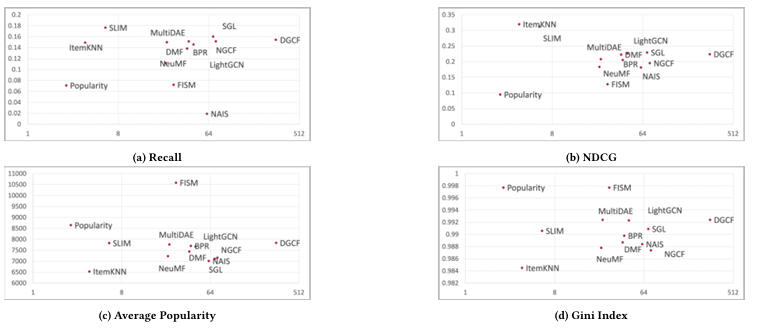
\includegraphics[width=\textwidth]{images/risultati-valutazione.png}
    \caption{Trade-off tra emissioni e performance con dataset Mind}
\end{figure}
\footnotesize
    \begin{equation*}
        \textit{emission} = \textit{CI}  \cdot \textit{PC}
    \end{equation*}
    \begin{equation*}
        \textit{CI} = \sum_{s \in S} \textit{e$_s$} \cdot \textit{p$_s$}
    \end{equation*}
\end{frame}

\begin{frame}{Regressore - Dataset e Modelli}
    \begin{wrapfigure}{r}{0.5\textwidth}
        \centering
        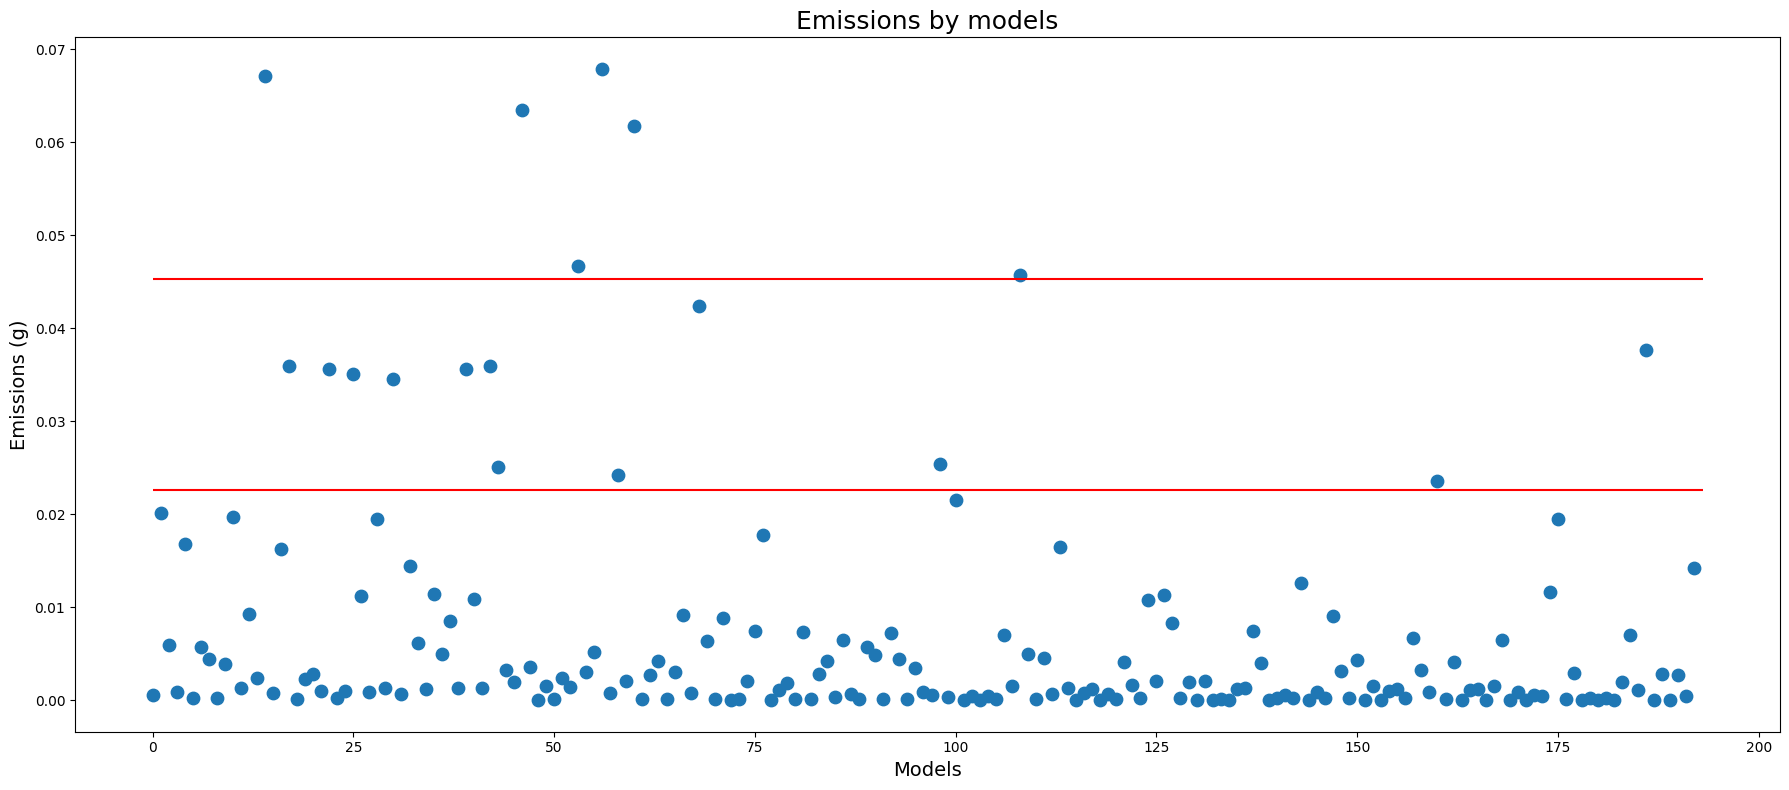
\includegraphics[width=0.5\textwidth]{images/situazione-attuale.png}
        \caption{Distribuzione emissioni nel Dataset}
    \end{wrapfigure}
    \small
    Il dataset del regressore è descritto dalle seguenti features di input:\textbf{n\_users}, \textbf{n\_items}, \textbf{n\_inter}, \textbf{sparsity}, \textbf{kg\_entities}, \textbf{kg\_relations}, \textbf{kg\_triples}, \textbf{kg\_items}, \textbf{cpu\_cores}, \textbf{ram\_size}, \textbf{is\_gpu}, \textbf{model\_name}, \textbf{model\_type}
    \vspace{1em}

    I modelli utilizzati sono:
     \textbf{Random Forest},\textbf{Decision Tree},\textbf{AdaBoost},\textbf{SVG}
\end{frame}
    


\begin{frame}{Regressore - Analisi dei risultati}
    \begin{figure}
    \centering
    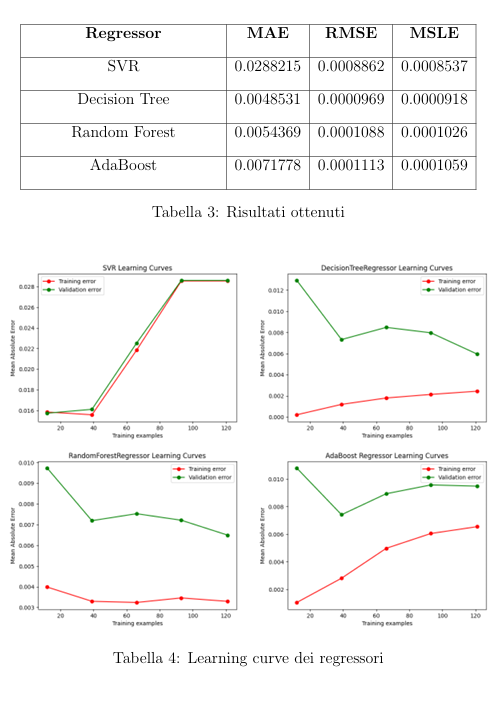
\includegraphics[height=0.8\textheight]{images/RegressorePrecedente.png}
    \caption{Risultati con split 70/30}
\end{figure}
\end{frame}
